\documentclass{tufte-handout}\usepackage[]{graphicx}\usepackage[]{color}
%% maxwidth is the original width if it is less than linewidth
%% otherwise use linewidth (to make sure the graphics do not exceed the margin)
\makeatletter
\def\maxwidth{ %
  \ifdim\Gin@nat@width>\linewidth
    \linewidth
  \else
    \Gin@nat@width
  \fi
}
\makeatother

\definecolor{fgcolor}{rgb}{0.345, 0.345, 0.345}
\newcommand{\hlnum}[1]{\textcolor[rgb]{0.686,0.059,0.569}{#1}}%
\newcommand{\hlstr}[1]{\textcolor[rgb]{0.192,0.494,0.8}{#1}}%
\newcommand{\hlcom}[1]{\textcolor[rgb]{0.678,0.584,0.686}{\textit{#1}}}%
\newcommand{\hlopt}[1]{\textcolor[rgb]{0,0,0}{#1}}%
\newcommand{\hlstd}[1]{\textcolor[rgb]{0.345,0.345,0.345}{#1}}%
\newcommand{\hlkwa}[1]{\textcolor[rgb]{0.161,0.373,0.58}{\textbf{#1}}}%
\newcommand{\hlkwb}[1]{\textcolor[rgb]{0.69,0.353,0.396}{#1}}%
\newcommand{\hlkwc}[1]{\textcolor[rgb]{0.333,0.667,0.333}{#1}}%
\newcommand{\hlkwd}[1]{\textcolor[rgb]{0.737,0.353,0.396}{\textbf{#1}}}%

\usepackage{framed}
\makeatletter
\newenvironment{kframe}{%
 \def\at@end@of@kframe{}%
 \ifinner\ifhmode%
  \def\at@end@of@kframe{\end{minipage}}%
  \begin{minipage}{\columnwidth}%
 \fi\fi%
 \def\FrameCommand##1{\hskip\@totalleftmargin \hskip-\fboxsep
 \colorbox{shadecolor}{##1}\hskip-\fboxsep
     % There is no \\@totalrightmargin, so:
     \hskip-\linewidth \hskip-\@totalleftmargin \hskip\columnwidth}%
 \MakeFramed {\advance\hsize-\width
   \@totalleftmargin\z@ \linewidth\hsize
   \@setminipage}}%
 {\par\unskip\endMakeFramed%
 \at@end@of@kframe}
\makeatother

\definecolor{shadecolor}{rgb}{.97, .97, .97}
\definecolor{messagecolor}{rgb}{0, 0, 0}
\definecolor{warningcolor}{rgb}{1, 0, 1}
\definecolor{errorcolor}{rgb}{1, 0, 0}
\newenvironment{knitrout}{}{} % an empty environment to be redefined in TeX

\usepackage{alltt}

%\documentclass{article}
\usepackage{graphicx}
%\setkeys{Gin}{width=\linewidth,totalheight=\textheight,keepaspectratio}
% Prints a trailing space in a smart way.
\usepackage{xspace}
\usepackage{hyperref}
\usepackage{amsmath}
\newcommand{\tthdump}[1]{#1}
\usepackage{makeidx}
\usepackage{tabularx}

%\makeindex

\begin{knitrout}
\definecolor{shadecolor}{rgb}{0.969, 0.969, 0.969}\color{fgcolor}\begin{kframe}


{\ttfamily\noindent\color{warningcolor}{\#\# Warning: No security definition has been found for the request}}\begin{verbatim}
## failed to load HTTP resource
\end{verbatim}


{\ttfamily\noindent\bfseries\color{errorcolor}{\#\# Error: 1: failed to load HTTP resource}}\end{kframe}
\end{knitrout}


\title{Buy On Gap trading report - S\&P 500}

\date{ 26 Nov 2013 }

\IfFileExists{upquote.sty}{\usepackage{upquote}}{}


\begin{document}
\maketitle

%\SweaveOpts{concordance=TRUE}
%\setkeys{Gin}{width=1.1\marginparwidth} %% Sweave

\section{Trade execution}
\subsection{Order executed}

% latex table generated in R 3.0.2 by xtable 1.7-1 package
% Wed Nov 27 05:10:31 2013
\begin{table}[ht]
\centering
\begin{tabular}{llrrrrrrr|r}
  \hline
 & Symbol & B.AvgPrc & B.Qty & S.AvgPrc & S.Qty & Profit & Comm. & Return \% & Closing Price \\ 
  \hline
1 & CNP & 23.96 & 4005 & 23.56 & 4005 & -1647.69 & 41.69 & -1.72 & 23.57 \\ 
   \hline
\end{tabular}
\end{table}



\subsection{Stock Portfolio}
% latex table generated in R 3.0.2 by xtable 1.7-1 package
% Wed Nov 27 05:10:31 2013
\begin{table}[ht]
\centering
\begin{tabular}{llrrr}
  \hline
 & Symbol & Quantity & Closing price & Market price \\ 
  \hline
1 & ***NO-ASSET*** &  &  &  \\ 
   \hline
\end{tabular}
\end{table}



\section{Trading Matrix}


% latex table generated in R 3.0.2 by xtable 1.7-1 package
% Wed Nov 27 05:10:31 2013
\begin{table}[ht]
\begin{tabular}{lr}
   \hline
Portofolio Amount: & 94573.82 \\ 
  Asset Amount: & 0.00 \\ 
  Bought Amount: & 95963.80 \\ 
  Sold   Amount: & 94357.80 \\ 
  Commission   : & 41.69 \\ 
  P/L incl Comm: & -1647.69 \\ 
  Ret incl Comm \%: & -1.71 \\ 
  S\&P 500 Ret \%: & 0.01 \\ 
   \hline
\end{tabular}
\caption{The commissions and daily returns are calculated based on the closed position.
The open position is present in the portofolio and assume closing on the next open market.
Portofolio amount is the open order with today closing price.} 
\end{table}



% \section{Trade Slippage}
% 
% <<slippage, echo = FALSE , results='asis'>>=
% 
% colnames(slippage) <- c('Symbol','Open Slippage %', 'Close Slippage %');
% print(xtable(slippage),floating=FALSE,);
% @


\title{Buy On Gap trading report - S\&P 600}
\maketitle

\section{Trade execution}
\subsection{Order executed}


% latex table generated in R 3.0.2 by xtable 1.7-1 package
% Wed Nov 27 05:10:31 2013
\begin{table}[ht]
\centering
\begin{tabular}{llrrrrrrr|r}
  \hline
 & Symbol & B.AvgPrc & B.Qty & S.AvgPrc & S.Qty & Profit & Comm. & Return \% & Closing Price \\ 
  \hline
1 & CBRL & 113.00 & 219 & 109.42 & 219 & -785.63 & 2.61 & -3.17 & 109.60 \\ 
  2 & RBCN & 9.26 & 2686 & 9.64 & 2686 & 991.07 & 27.31 & 3.98 & 9.64 \\ 
  3 & RLI & 100.06 & 246 & 100.83 & 246 & 185.77 & 2.89 & 0.75 & 100.85 \\ 
   \hline
\end{tabular}
\end{table}



\subsection{Stock Portfolio}
% latex table generated in R 3.0.2 by xtable 1.7-1 package
% Wed Nov 27 05:10:31 2013
\begin{table}[ht]
\centering
\begin{tabular}{llrrr}
  \hline
 & Symbol & Quantity & Closing price & Market price \\ 
  \hline
1 & ***NO-ASSET*** &  &  &  \\ 
   \hline
\end{tabular}
\end{table}



\section{Trading Matrix}

% latex table generated in R 3.0.2 by xtable 1.7-1 package
% Wed Nov 27 05:10:31 2013
\begin{table}[ht]
\begin{tabular}{lr}
   \hline
Portofolio Amount: & 99034.53 \\ 
  Asset Amount: & 0.00 \\ 
  Bought Amount: & 74236.18 \\ 
  Sold   Amount: & 74660.20 \\ 
  Commission   : & 32.81 \\ 
  P/L incl Comm: & 391.21 \\ 
  Ret incl Comm \%: & 0.40 \\ 
  S\&P 600 Ret \%: & 0.60 \\ 
   \hline
\end{tabular}
\caption{The commissions and daily returns are calculated based on the closed position.
The open position is present in the portofolio and assume closing on the next open market.
Portofolio amount is the open order with today closing price.} 
\end{table}



% \section{Trade Slippage}
% 
% <<slippage_sp600, echo = FALSE , results='asis'>>=
% 
% colnames(slippage) <- c('Symbol','Open Slippage %', 'Close Slippage %');
% print(xtable(slippage),floating=FALSE,);
% @

\newpage
\section{News}

%\begin{margintable}

% latex table generated in R 3.0.2 by xtable 1.7-1 package
% Wed Nov 27 05:10:31 2013
\begin{tabularx}{\textwidth}{rX}
  \hline
 & CNP \\ 
  \hline
1 &  CenterPoint Energy, Inc. (NYSE:CNP) today announced that David M. McClanahan, 64, will step down as president and chief executive officer and as a member of the company's board of directors, ...  \\ 
  2 &  In April, CenterPoint reached an agreement with XTO Energy Inc., a subsidiary of Exxon Mobil Corp., (NYSE: XOM), to gather XTO's crude oil production through a new pipeline system in North Dakota's Bakken shale.  \\ 
  3 &  Shares in CenterPoint Energy Inc. edged higher on Monday, tracking gains in the broader market. The company's shares closed the day 0.16\% higher at \$24.45, after vacillating between \$24.22 and \$24.58.  \\ 
  4 &  Our earnings press release and Form 10-Q are posted on our website, centerpointenergy.com, under the Investors section. I remind you that any projections or forward-looking statements made during this call are subject to the cautionary statements on ...  \\ 
  5 &  CenterPoint Energy Inc. (NYSE: CNP) plans to take its Enable Midstream Partners side of the business public by 2014. In an earnings conference call to investors, CenterPoint outlined its strategy for Enable, an \$11 billion natural gas midstream ...  \\ 
  6 &  Market Buzz Report, which provides regular updates on penny stocks, releases critical updates for CenterPoint Energy, Inc.(NYSE:CNP), Abercrombie \& Fitch Co.(NYSE:ANF), Himax Technologies, Inc. (NASDAQ:HIMX), Wal-Mart Stores, Inc.(NYSE:WMT), ...  \\ 
  7 &  CenterPoint Energy logo CenterPoint Energy (NYSE:CNP) declared a quarterly dividend on Wednesday, October 23rd, Analyst Ratings Network.  \\ 
  8 &  Wall Street Pennies is engaged in providing the most up to date and useful information on the Best Penny Stocks that are poised to breakout.  \\ 
  9 &  CenterPoint Energy, Inc. (NYSE:CNP) operates as a public utility holding company in the United States is currently down (-6.84\%) on 8,134,977 shares traded after CenterPoint Energy, OGE Energy and ArcLight Capital's Enable Midstream Partners Filed ...  \\ 
  10 &  Shares of CenterPoint Energy (NYSE:CNP) traded down 5.69\% on Tuesday, hitting \$23.455. 18,838,820 shares of the company's stock traded hands. CenterPoint Energy has a 52-week low of \$18.79 and a 52-week high of \$25.65. The stock's 50-day moving ...  \\ 
   \hline
\end{tabularx}


%\end{margintable}

\newpage
\section{Individual contract}
\begin{fullwidth}
\begin{knitrout}
\definecolor{shadecolor}{rgb}{0.969, 0.969, 0.969}\color{fgcolor}\begin{kframe}


{\ttfamily\noindent\bfseries\color{errorcolor}{\#\# Error: chartSeries requires an xtsible object}}\end{kframe}
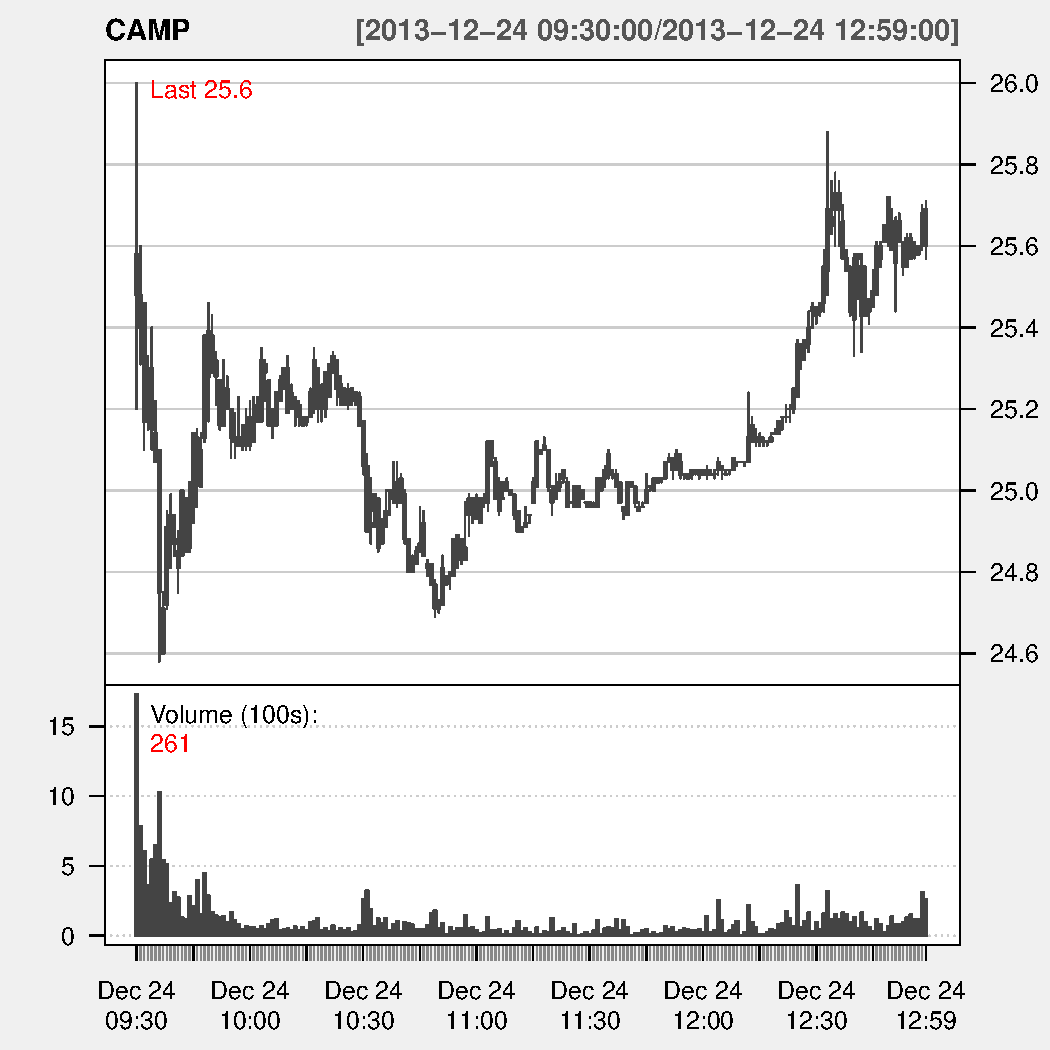
\includegraphics[width=\maxwidth]{/home/jhleong/dev/R/buy_on_gap/BuyOnGap_report/figure/price_chart} 

\end{knitrout}


\end{fullwidth}
\end{document}
